\documentclass[a4paper,10pt]{article}
\usepackage[utf8]{inputenc}
\usepackage{url}
\usepackage{indentfirst}


\title{IF738 - Redes de Computadores}
\author{Karen Samara}
\date{Novembro 2019}

\usepackage{natbib}
\usepackage{graphicx}

\begin{document}

\maketitle

\section{Introdução} 
    Redes de Computadores é uma área que abrange tudo que se relaciona à comunicação entre computadores, chamados hosts, que vai desde a parte física (hardware), como cabeamento e configuração de dispositivos importantes e auxiliares à essa comunicação (switches, hubs, etc...), à partes não-físicas (software), como a programação de redes sem uso de fios (wireless) e a configuração e uso de protocolos de redes. 
    \par
    Foram criados, então, modelos de referências divididos em camadas, TCP/IP \cite{link3} com 4 camadas e o modelo OSI \cite{link2} com 7 camadas, para padronizar e facilitar a conexão entre computadores, onde cada camada possui sua função e seus protocolos.

\begin{figure}[h!]
\centering
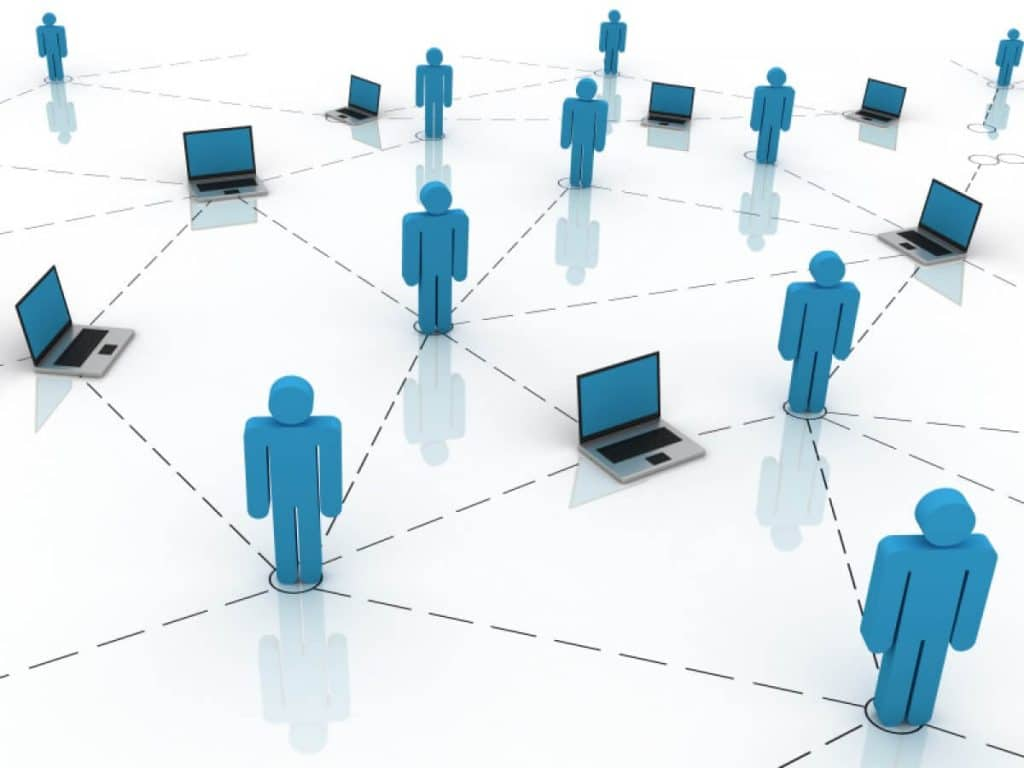
\includegraphics[scale=0.1]{computer-network.jpg}
\caption{Rede de computadores e pessoas \cite{imagem1}}
\label{fig:computer-network}
\end{figure}

\section{Relevância}
    As redes de computadores estão presentes em todos os segmentos, tendo se tornado vitais para praticamente qualquer área do mercado. Seu surgimento melhorou a comunicação e o acesso à informação em governos, empresas, escolas e outras instituições, fazendo com que seus trabalhos sejam mais eficientes e ágeis.\cite{link4}  
    \\ \par
Pontos positivos:
\begin{itemize}
    \item Criação de mais oportunidades para segurança de informações;
    \item Possibilidade de expansão do potencial das redes;
    \item Possibilidade de trabalhar em diversas áreas do mercado.
\end{itemize}

\section{Relação com outras disciplinas}
    Redes de Computadores tem relação com todos os componentes eletivos referentes a redes e sistemas distribuídos, além de, Banco de Dados, pois ambas áreas trabalham com fluxo de dados e controlam acesso a informações sigilosas, se relaciona também com Lógica de Programação, pois assim como na área de programação, em Redes de Computadores, também é necessário aprender a lidar com problemas e resolvê-los, e, por fim, Inglês para Computação, pois linguagem técnica é muito utilizada e importante para o entendimento de grande parte da área de Redes de Computadores.

\nocite{link1,link5}
\bibliographystyle{unsrt}
\bibliography{ksbs}
\end{document}
